\chapauthor{Ковалёв М.В.\\Крощенко А.А.\\Головко В.А.}
\chapter{Конвергенция и интеграция искусственных нейронных сетей с базами знаний в интеллектуальных компьютерных системах нового поколения}
\chapauthortoc{Ковалёв М.В.\\Крощенко А.А.\\Головко В.А.}
\label{chapter_ann}

\abstract{В последнее десятилетие все больше назревает необходимость в разработке гибридных интеллектуальных систем. В контексте этого особое значение приобретают системы, разработанные с использованием семантической технологии (например, \scnkeyword{Технологии OSTIS}) и искусственных нейронных сетей (\scnkeyword{и.н.с.}). Такие гибридные системы обладают достоинствами, которые недостижимы при использовании отдельных технологий. С одной стороны, здесь используются нейронные сети, которые могут работать с неструктурированными и плохо формализованными данными. С другой стороны, применяются семантические технологии, благодаря которым можно объяснить работу любого ``черного'' ящика. Все это формирует серьезную основу для разработки систем, способных не только к эффективной обработке данных, но и к интерпретации получаемых на каждом этапе результатов.} 

\section{Модели искусственных нейронных сетей, используемых в ostis-системах}

Преимущество \scnkeyword{и.н.с.} заключается в том, что они могут работать с неструктурированными данными.
Главный недостаток \scnkeyword{и.н.с.} -- это отсутствие понятной человеку обратной связи, которую можно было бы назвать цепочкой
рассуждений, т.е. можно сказать, что \scnkeyword{и.н.с.} работают по принципу ``черного ящика'' (\scncite{gastelvecchi2016}).

Сложность современных интеллектуальных систем, использующих нейросетевые модели, а также большой объём обрабатываемых ими данных обуславливают необходимость объяснения и мониторинга механизмов их работы с целью оценки их деятельности и ее оптимизации.

В связи с этим актуальность приобретает разработка нейросимволических подходов (описанных, например, в работе \scncite{nesy1}), в частности, подходов по интеграции \scnkeyword{и.н.с.} и баз знаний, использующих онтологии. Такие интегрированные системы способны сочетать работу \scnkeyword{и.н.с.} по извлечению скрытых закономерностей из массива данных с возможностью их семантической интерпретации чисто символическими подходами ИИ. Это позволяет более точно описать свойства \scnkeyword{и.н.с.}, ее состояния, что в свою очередь делает возможным приоткрыть завесу неопределенности над процессами, скрытыми в ``черном ящике'' (\scncite{ann_ostis2018}).

Можно выделить два основных направления интеграции \scnkeyword{и.н.с.} с базами знаний:

\begin{itemize}
	\item построение интеллектуальных систем, использующих нейросетевые методы наравне с другими имеющимися в системе методами для решения задач или подзадач системы. Такие системы смогут учитывать семантику решаемых задач на более высоком уровне, что сделает решение этих задач структурированными и понятным.

	\item построение интеллектуальной среды по разработке, обучению и интеграции различных \scnkeyword{и.н.с.}, совместимых с базами знаний через представление структур \scnkeyword{и.н.с.} с помощью онтологического подхода и их интерпретацию средствами представления знаний.
	
	\item исследование влияния входных данных на выход нейронных сетей с формулированием правил, которые могут быть погружены в БЗ.
\end{itemize}

Такая среда предоставит возможности интроспекции \scnkeyword{и.н.с.}, сохранения состояний \scnkeyword{и.н.с.} после обучения и реконфигурации сети с целью улучшения ее качеств.

Таким образом, станет возможным проводить более глубокий анализ работы \scnkeyword{и.н.с.}. С другой стороны, формальное описание знаний в рамках предметной области \scnkeyword{и.н.с.} уменьшит порог вхождения разработчиков в теорию методов решения задач с помощью \scnkeyword{и.н.с.}

Данный раздел посвящен предметной области и онтологии искусственных нейронных сетей, используемых в ostis-системах

\subsection{Синтаксис моделей искусственных нейронных сетей, используемых в ostis-системах}

Используя \textit{SC-код}, искусственную нейронную сеть можно определить как 

\begin{SCn}
	\scnheader{искусственная нейронная сеть}
	\scnidtf{и.н.с.}
	\scnidtf{множество искусственных нейронных сетей}
	\scnidtf{нейронная сеть}
	\scntext{пояснение}{Cовокупность нейронных элементов и связей между ними (\scncite{Golovko2017}).
	Искусственная нейронная сеть состоит из \textbf{\textit{формальных нейронов}}, которые связаны между собой посредством \textbf{\textit{синаптических связей}}. Нейроны организованы в \textbf{\textit{слои}}. Каждый нейрон слоя принимает сигналы с входящих в него синаптических связей, обрабатывает их единым образом с помощью заданной ему или всему слою \textbf{\textit{функции активации}} и передает результат на следующий слой нейронных элементов. Структура и характеристики слоев определяют порядок обработки информации в нейронной сети.}
\end{SCn}

Пример архитектуры и.н.с. представлен на рисунке \textit{\nameref{fig:nn_example}}.

\begin{figure}[H]
	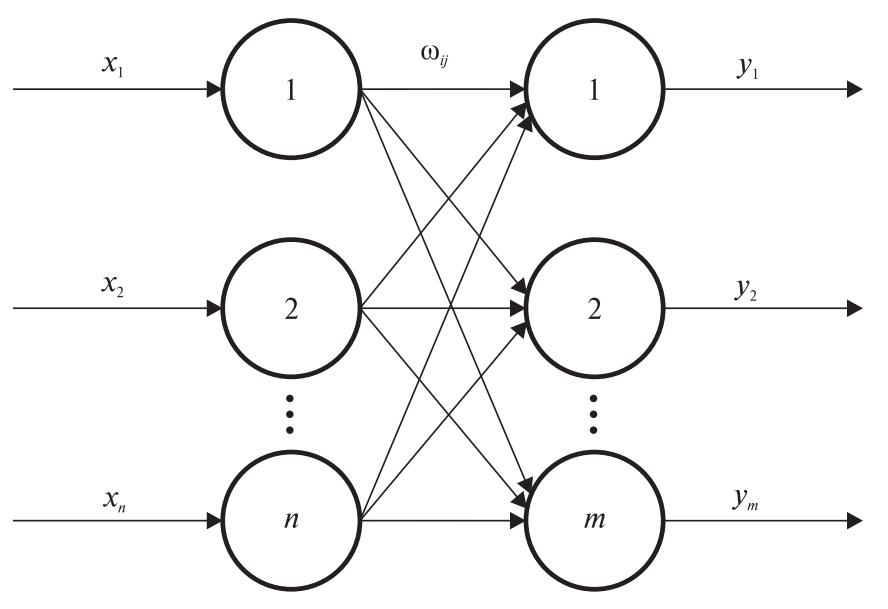
\includegraphics[scale=0.3]{author/part3/figures/neural_network.png}
	\caption{Пример архитектуры и.н.с.}
	\label{fig:nn_example}
\end{figure}

	Такая формулировка предполагает существование определенной нейросетевой архитектуры, которая определяет структурную конфигурацию модели.
	
	Рассмотрим архитектурные компоненты подробнее.

\begin{SCn}
	\scnheader{формальный нейрон}
	\scnidtf{искусственный нейрон}
	\scnidtf{нейрон}
	\scnidtf{ф.н.}
	\scnidtf{нейронный элемент}
	\scnidtf{множество нейронов искусственных нейронных сетей}
	\scnidtf{математическая модель биологического нейрона}
	\scnsubset{искусственная нейронная сеть}
	\scntext{пояснение}{Основной элемент \scnkeyword{искусственной нейронной сети}, применяющий свою \scnkeyword{функцию активации} (\scncite{Golovko2017}) к сумме произведений входных сигналов на весовые коэффициенты:
	\begin{equation*}
		y = F\left(\sum_{i=1}^{n} w_ix_i - T\right) = F(WX - T)
	\end{equation*}
	где $X = (x_1,x_2,...,x_n)^{T}$ -- вектор входного сигнала; $W - (w_1,w_2,...,w_n)$ -- вектор весовых коэффициентов; \textit{T} -- пороговое значение;
	\textit{F} -- \scnkeyword{функция активации}.}

	\scntext{примечание}{Отдельный формальный нейрон является искусственной нейронной сетью с одним нейроном в единственном слое.}
\end{SCn}

Пример описания одного нейрона в SCg представлен на рисунке \textit{\nameref{fig:nn_scg}}.

\begin{figure}[H]
	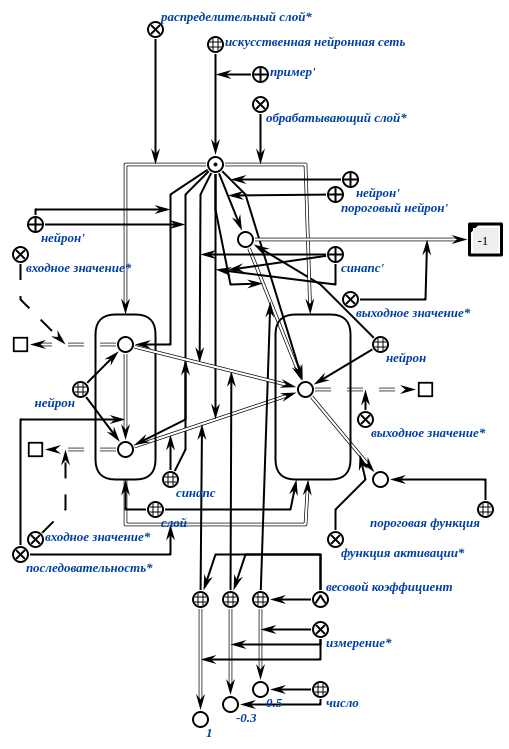
\includegraphics[scale=0.8]{author/part3/figures/neural_network_scg.png}
	\caption{Представление одного нейрона в SCg}
	\label{fig:nn_scg}
\end{figure}

Формальные нейроны могут быть классифицированы следующим образом:

\begin{itemize}
		\item полносвязный формальный нейрон -- нейрон, у которого есть полный набор связей с нейронами предшествующего слоя. Oтдельный обрабатывающий элемент \scnkeyword{и.н.с.}, выполняющий функциональное преобразование взвешенной суммы элементов вектора входных значений с помощью \scnkeyword{функции активации}
	 \item сверточный формальный нейрон -- отдельный обрабатывающий элемент \scnkeyword{и.н.с.}, выполняющий функциональное преобразование результата операции свертки матрицы входных значений с помощью \scnkeyword{функции активации}. Сверточный \scnkeyword{формальный нейрон} может быть представлен полносвязным \scnkeyword{формальным нейроном}.
	\item рекуррентный \scnkeyword{формальный нейрон} -- нейрон, имеющий обратную связь с самим собой или с другими нейронами \scnkeyword{и.н.с.}
\end{itemize}

Схематически формальный нейрон можно представить в виде следующей модели (рисунок \textit{\nameref{fig:formal_neuron}}).

\begin{figure}[H]
	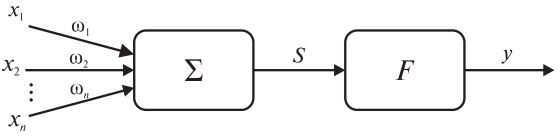
\includegraphics[scale=0.8]{author/part3/figures/formal_neuron.png}
	\caption{Формальный нейрон}
	\label{fig:formal_neuron}
\end{figure}

Определим понятие \scnkeyword{синаптическая связь} и \scnkeyword{слой и.н.с.}:

\begin{SCn}
	\scnheader{синаптическая связь}
	\scnidtf{синапс}
	\scnsubset{ориентированная пара}
	\scntext{пояснение}{ориентированная пара, первым компонентом которой является нейрон, из
	которого исходит сигнал, а вторым компонентом -- нейрон, который принимает этот сигнал}
\end{SCn}


\begin{SCn}
	\scnheader{слой и.н.с.}
	\scnidtf{слой}
	\scnidtf{слой искусственной нейронной сети}
	\scnidtf{множество слоев искусственных нейронных сетей}
	\scnsubset{искусственная нейронная сеть}
	\scntext{пояснение}{множество нейронных элементов, на которые в каждый такт времени
		параллельно поступает информация от других нейронных элементов сети (\scncite{Golovko2017})}
	\scntext{пояснение}{множество формальных нейронов, осуществляющих параллельную независимую обработку вектора или матрицы входных значений}
	\scntext{примечание}{отдельный слой является искусственной нейронной сетью с одним слоем}
\end{SCn}

Здесь следует отметить принципиальную важность последнего примечания. Один \scnkeyword{формальный нейрон}  уже является нейронной сетью, поскольку над ним можно производить все основные операции, которые производятся над ``большой'' {и.н.с.} (его можно обучить и использовать для решения определенной задачи).

\scnkeyword{Слои и.н.с.} могут быть классифицированы следующим образом (по признаку операции, осуществляемой слоем):
\begin{itemize}
		\item полносвязный слой и.н.с. -- слой, в котором каждый нейрон является полносвязным
		\item сверточный слой и.н.с. -- слой, в котором каждый нейрон является сверточным
		\item слой и.н.с. нелинейного преобразования -- слой, осуществляющий нелинейное преобразование входных данных
		\item dropout слой и.н.с. -- слой, реализующий технику регуляризации dropout
		\item pooling слой и.н.с. -- подвыборочный слой
		\item слой и.н.с. батч-нормализации
\end{itemize}


Как правило, слой нелинейного преобразования  выделяется в отдельный слой только в программных реализациях. Фактически он рассматривается как финальный этап расчета выходной активности любого нейрона -- применение \scnkeyword{функции активации}.

Dropout-слой функционирует только во время обучения \scnkeyword{и.н.с.} Поскольку полносвязные слои имеют большое количество настраиваемых параметров, они подвержены эффекту \scnkeyword{переобучения}. Один из способов устранить такой негативный эффект -- выполнить частичный отсев результатов на выходе полносвязного слоя. На этапе обучения техника dropout позволяет отбросить выходную активность некоторых нейронов с определенной, заданной вероятностью. Выходная активность ``отброшенных'' нейронов полагается равной нулю.

Назначение подвыборочного слоя -- в осуществлении уменьшения размерности входных данных.

Нужно отметить, что данный перечень неполный -- разновидности \scnkeyword{слоев и.н.с.} появляются практически в каждой заслуживающей внимания публикации по нейросетевым алгоритмам и на текущий момент их существует достаточно много, однако, как правило, при построении более традиционных архитектур ограничиваются только приведенными вариантами слоев.

\scnkeyword{Слои и.н.с.} также могут быть классифицированы по исполняемой роли в рамках архитектуры (место в последовательности \scnkeyword{слоев и.н.с.}).

Так, например, слой, расположенный первым, называется распределяющим. Слои, расположенные далее, за исключением последнего, называются обрабатывающими. Наконец, последний слой носит название выходного \scnkeyword{слоя и.н.с.}

Наконец, последний архитектурный компонент \scnkeyword{и.н.с.} -- это функция активации:

\begin{SCn}
	\scnheader{функция активации*}
	\scnidtf{функция активации нейрона*}
	\scniselement{неролевое отношение}
	\scniselement{бинарное отношение}
	\scntext{пояснение}{неролевое отношение, связывающее формальный нейрон с функцией, результат
		применения которой к \textbf{\textit{взвешенной сумме нейрона}} определяет его \textbf{\textit{выходное значение}}.}
	%\scnrelfrom{область определения}{
		
	%}
    %\scnreltoset{объединение}{формальный нейрон;функция}
	\scnrelfrom{первый домен}{формальный нейрон}
	\scnrelfrom{второй домен}{функция}
\end{SCn}

Перечислим некоторые, наиболее известные и применяемые типы функций активации:
\begin{itemize}
	\item линейная функция\\
	\scntext{формула}{
		\begin{equation*}
			y = kS
		\end{equation*}
		где \textit{k} -- коэффициент наклона прямой, \textit{S} -- в.с.
	}
	\item пороговая функция\\
	\scntext{формула}{
		\begin{equation*}
			y = sign(S) =
			\begin{cases}
				1, S > 0,\\
				0, S \leq 0
			\end{cases}
		\end{equation*}
	}
	\item сигмоидная функция\\
	\scntext{формула}{
		\begin{equation*}
			y = \frac{1}{1+e^{-cS}}
		\end{equation*}
		где \textit{с} > 0 -- коэффициент, характеризующий ширину сигмоидной функции по оси абсцисс, \textit{S} -- в.с.
	}
	\item функция гиперболического тангенса\\
	\scntext{формула}{
		\begin{equation*}
			y = \frac{e^{cS}-e^{-cS}}{e^{cs}+e^{-cS}}
		\end{equation*}
		где \textit{с} > 0 -- коэффициент, характеризующий ширину сигмоидной функции по оси абсцисс, \textit{S} -- в.с.
	}
	\item функция softmax\\
	\scntext{формула}{
		\begin{equation*}
			y_j = softmax(S_j) = \frac{e^{S_j}}{\sum_{j} e^{S_j}}
		\end{equation*}
		где $S_j$ -- в.с. \textit{j}-го выходного нейрона
	}
	\item функция ReLU\\
	\scntext{формула}{
		\begin{equation*}
			y = F(S) =
			\begin{cases}
				S, S > 0,\\
				kS, S \leq 0
			\end{cases}
		\end{equation*}
		где \textit{k} = 0 или принимает небольшое значение, например, 0.01 или 0.001.
	}
\end{itemize}

\subsection{Денотационная семантика моделей искусственных нейронных сетей, используемых в ostis-системах}

\subsection{Операционная семантика моделей искусственных нейронных сетей, используемых в ostis-системах}

Рассмотрим основные действия, выполняемые с и.н.с.

\begin{itemize}
	\item действие конфигурации и.н.с.
	\begin{itemize}
		\item действие создания и.н.с.
		\item действие редактирования и.н.с.
		\item действие удаления и.н.с.
		\item действие конфигурации слоя и.н.с.
		\begin{itemize}
			\item действие добавления слоя в и.н.с.
			\item действие редактирования слоя и.н.с.
			\item действие удаления слоя и.н.с.
			\item действие установки функции активации нейронов слоя и.н.с.
			\item действие конфигурации нейрона в слое и.н.с.
			\begin{itemize}
				\item действие добавления нейрона в слой и.н.с.
				\item действие редактирования нейрона в слое и.н.с.
				\item действие удаления нейрона из слоя и.н.с.
				\item действие установки функции активации нейрона в слое и.н.с.
			\end{itemize}
		\end{itemize}
	\end{itemize}
	\item действие конфигурации настраиваемых параметров и.н.с.
	\item действие интерпретации и.н.с.
\end{itemize}

Первый тип разновидностей действий относится к архитектурному изменению и.н.с., который влияет на ее структуру. Второй тип связан с начальной инициализацией настраиваемых параметров нейронной сети и ее обучением. Наконец третий тип действий связан с интерпретированием результатов, получаемых нейронной сетью и, в целом, может рассматриваться как действие по использованию (применению) и.н.с. для решения конкретной задачи.

Действия по обработке и.н.с. осуществляет соответствующий коллектив агентов. 

Так как в результате действий по обработке и.н.с. объект этих действий, конкретная и.н.с., может существенно меняться (меняется конфигурация сети, ее весовые коэффициенты), то и.н.с. представляется в базе знаний как темпоральное объединение всех ее версий. Каждая версия является  \scnkeyword{и.н.с.} и темпоральной сущностью. На множестве этих темпоральных сущностей задается темпоральная последовательность с указанием первой и последней версии. Для каждой версии описываются специфичные знания.

Общие для всех версий знания описываются для и.н.с, являющейся темпоральным объединением всех версий (рисунок \textit{\nameref{fig:temporal_neural_network_scg}})

\begin{figure}[H]
	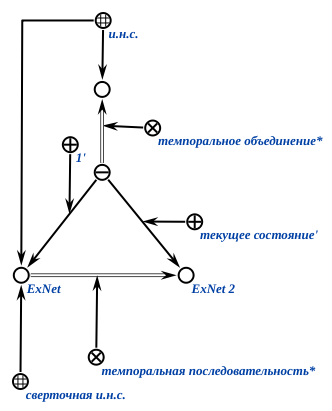
\includegraphics[scale=0.8]{author/part3/figures/temporal_neural_network_scg.png}
	\caption{Темпоральность нейронной сети}
	\label{fig:temporal_neural_network_scg}
\end{figure}

Далее более подробно рассмотрим действие по обучению и.н.с. и сделаем обзор основных методов, применяемых для обучения.

Действие обучения  \scnkeyword{и.н.с.} -- действие, в ходе которого реализуется определенный метод обучения  \scnkeyword{и.н.с.} с заданными параметрами обучения  \scnkeyword{и.н.с.}, методом оптимизации и функцией потерь.

При обучении возможно возникновение следующих проблем:

\begin{itemize}
	\item Переобучение -- проблема, возникающая при обучении  \scnkeyword{и.н.с.}, заключающаяся в том,
	что сеть хорошо адаптируется к паттернам входной активности из обучающей выборки, при этом теряя способность к обобщению.
	Переобучение возникает из-за применения неоправданно сложной модели при обучении  \scnkeyword{и.н.с.} Это происходит,
	когда количество настраиваемых параметров и.н.с. намного больше размера обучающей выборки. Возможные
	варианты решения проблемы заключаются в упрощении модели, увеличении выборки, использовании регуляризации
	(параметр регуляризации, техника dropout и т.д.).\\
	Обнаружение переобученности сложнее, чем недообученности. Как правило, для этого применяется
	кросс-валидация на валидационной выборке, позволяющая оценить момент завершения процесса обучения.
	Идеальным вариантом является достижение баланса между переобученностью и недообученностью.
	
	\item Недообучение -- проблема, возникающая при обучении  \scnkeyword{и.н.с.}, заключающаяся в том,
	что сеть дает одинаково плохие результаты на обучающей и контрольной выборках.
	Чаще всего такого рода проблема возникает при недостаточном времени, затраченном на обучение модели.
	Однако это может быть вызвано и слишком простой архитектурой модели либо малым размером обучающей
	выборки. Соответственно решение, которое может быть принято ML-инженером, заключается в устранении
	этих недостатков: увеличение времени обучения, использование модели с большим числом настраиваемых
	параметров, увеличение размера обучающей выборки, а также уменьшение регуляризации и более тщательный
	отбор признаков для обучающих примеров.
\end{itemize}

Методом обучения \scnkeyword{и.н.с.} называется процесс итеративного поиска оптимальных значений настраиваемых параметров и.н.с., минимизирующих некоторую заданную функцию потерь.

Стоит отметить, что хотя целью применения метода обучения является минимизация функции потерь, ``полезность'' полученной после обучения модели можно оценить только по достигнутому уровню ее обобщающей способности.

Методы обучения могут быть поделены на две большие группы -- \textit{\textbf{методы обучения с учителем}} и \textit{\textbf{методы обучения без учителя}} (контролируемый и неконтролируемый методы обучения).

Метод обучения с учителем -- метод обучения с использованием заданных целевых переменных.

Одним из методов обучения с учителем является метод обратного распространения ошибки.

Приведем его описание в виде алгоритма:

\begin{algorithm}[H]
	\KwData{$X$ -- данные, $E_t$ -- желаемый отклик (метки), $E_m$ -- желаемая ошибка (в соответствии с выбранной функцией потерь)}
	\KwResult{обученная нейронная сеть \textit{Net}}
	инициализация весов \textit{W} и порогов \textit{T};\\
	\Repeat{$E<E_m$}{
		\ForEach{$x \in X$, $e \in E_t$}{
			фаза прямого распространения сигнала: вычисляются активации для всех слоев и.н.с.;\\
			фаза обратного распространения ошибки: вычисляются ошибки для последнего слоя и всех предшествующих слоев;\\
			изменение настраиваемых параметров и.н.с. в соответствии с вычисленными ошибками;\\
		}
		вычисление общей ошибки E на данной эпохе;
	}
\end{algorithm}

Метод обратного распространения ошибки использует заданный метод оптимизации и заданную функцию потерь для реализации фазы обратного распространения ошибки и изменения настраиваемых параметров и.н.с. Одним из самых распространенных методов оптимизации является метод стохастического градиентного спуска. Приведенный метод используется для реализации последовательного варианта обучения.

Следует также отметить, что несмотря на то, что метод отнесен к методам обучения с учителем, в случае
его использования для обучения автокодировщиков в классических публикациях он рассматривается как
метод обучения без учителя, поскольку в данном случае размеченные данные отсутствуют.

\textbf{\textit{Метод обучения без учителя}} -- метод обучения без использования заданных целевых переменных (в режиме самоорганизации)

В ходе выполнения алгоритма метода обучения без учителя выявляются полезные структурные свойства
набора. Неформально его понимают как метод для извлечения информации из распределения, выборка для которого
не была вручную аннотирована человеком (\scncite{Goodfellow2017}). Метод обучения без учителя может рассматриваться как вспомогательный метод для начальной инициализации настраиваемых параметров и.н.с. В этом случае он является методом предобучения.

Среди методов, применяемых для оптимизации целевой функции можно выделить следующие:

\begin{itemize}
	\item SGD (стохастический градиентный спуск): в данном методе корректировка настраиваемых параметров и.н.с. выполняется в направлении максимального уменьшения функции стоимости, т.е. в направлении, противоположном вектору градиента функции потерь (\scncite{Haykin2006})
	\item метод Нестерова: Обучение методом стохастического градиентного спуска иногда происходит очень медленно. Импульсный метод позволяет ускорить обучение, особенно в условиях высокой кривизны, небольших, но устойчивых градиентов или зашумленных градиентов. В импульсном методе вычисляется экспоненциально затухающее скользящее среднее прошлых градиентов и продолжается движение в этом направлении. Метод Нестерова является вариантом импульсного алгоритма, в котором градиент вычисляется после применения текущей скорости (\scncite{Goodfellow2017})
	\item AdaGrad: Данный метод по отдельности адаптирует скорости обучения всех настраиваемых параметров и.н.с., умножая их на коэффициент, обратно пропорциональный квадратному корню из суммы всех прошлых значений квадрата градиента (\scncite{Duchi2011})
	\item RMSProp: Данный метод является модификацией AdaGrad, которая позволяет улучшить его поведение в невыпуклом случае путем изменения способа агрегирования градиента на экспоненциально взвешенное скользящее среднее. Использование экспоненциально взвешенного скользящего среднего гарантирует повышение скорости сходимости после обнаружения выпуклой впадины, как если бы внутри этой впадины алгоритм AdaGrad был инициализирован заново (\scncite{Goodfellow2017})
	\item Adam: Данный метод можно рассматривать как комбинацию RMSProp и AdaGrad (\scncite{Kingma2014}). Помимо усредненного первого момента, данный метод использует усредненное значение вторых моментов градиентов
\end{itemize} 

Отметим, что успешность применения методов оптимизации зависит главным образом от знакомства пользователя с соответствующим алгоритмом (\scncite{Goodfellow2017}.

Еще одним важным компонентом, влияющим на процесс обучения, является используемая функция потерь.

\textbf{\textit{Функция потерь} -- функция, используемая для вычисления ошибки, рассчитываемой как разница между фактическим эталонным значением и прогнозируемым значением, получаемым и.н.с.}

Среди функций потерь, используемые в качестве целевых функций для применяемого метода оптимизации, можно выделить:

\begin{itemize}
	\item MSE -- средняя квадратичная ошибка\\
		\begin{equation*}
			MSE = \frac{1}{L} \sum_{l=1}^L \sum_{i=1}^m (y_i^l - e_i^l)^2
		\end{equation*}
		где $y_i^l$ -- прогноз модели, $e_i^l$ -- ожидаемый (эталонный) результат, \textit{m} -- размерность выходного вектора, \textit{L} -- объем обучающей выборки.

	\item BCE -- бинарная кросс-энтропия\\
	\begin{equation*}
		BCE = - \sum_{l=1}^L (e^l \log(y^l) + (1 - e^l)\log(1 - y^l))
	\end{equation*}
	где $y^l$ -- прогноз модели, $e^l$ -- ожидаемый (эталонный) результат: \textit{0} или \textit{1}, \textit{L} -- объем обучающей выборки.
	\item MCE -- мультиклассовая кросс-энтропия\\
	\begin{equation*}
		MCE = - \sum_{l=1}^L \sum_{i=1}^m e_{i}^l \log(y_{i}^l)
	\end{equation*}
	где $y_{i}^l$ -- прогноз модели, $e_i^l$ -- ожидаемый (эталонный результат), \textit{m} -- размерность выходного вектора
\end{itemize}

Отметим, что для бинарной кросс-энтропии в выходном слое и.н.с. будет находиться один нейрон, а для для мультиклассовой кросс-энтропии количество нейронов в выходном слое и.н.с. совпадает с количеством классов.

Для решения задачи классификации рекомендуется использовать бинарную или мультиклассовую кросс-энтропийную функцию потерь, для решения задачи регрессии рекомендуется использовать среднюю квадратичную ошибку.

Действие обучения и.н.с. можно проиллюстрировать следующим изображением \textit{\nameref{fig:ann_training_nn_scg}}.

\begin{figure}[H]
	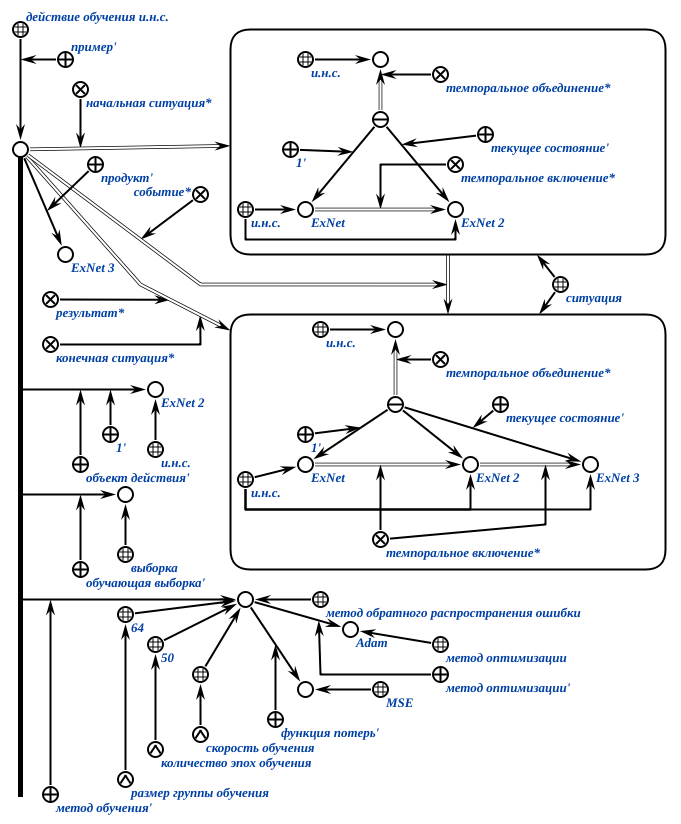
\includegraphics[scale=0.8]{author/part3/figures/ann_training_nn_scg.png}
	\caption{Действие обучения и.н.с.}
	\label{fig:ann_training_nn_scg}
\end{figure}

\section{Логико-семантическая модель ostis-системы автоматизации проектирования искусственных нейронных сетей, семантически совместимых с базами знаний ostis-систем}
\section{Применение глубоких нейронных сетей в интеллектуальных компьютерных системах нового поколения}

Хотя строгого определения понятия глубокая нейронная сеть не существует, ее можно определить как \scnkeyword{и.н.с.} произвольной архитектуры, имеющую более двух скрытых слоев нейронных элементов. В настоящий момент глубокой фактически можно считать любую \scnkeyword{и.н.с.}, на которую не накладывается условие ограничение глубины. Долгое время нейронные сети с более чем двумя скрытыми слоями не изучались и не находили практического применения по причине того, что их обучение классическими подходами (в частности, алгоритмом обратного распространения ошибки) было неэффективно и не приводило к желаемым результатам. Неэффективность была прежде всего связана с проблемой <<исчезающего градиента>>, которая проявляется в том, что при обучении нейронной сети с большим количеством слоев методом обратного распространения ошибки значения градиентов весовых коэффициентов первых слоев сети быстро становятся близкими к нулю, приводя к тому, что весовые коэффициенты таких слоев практически не изменяются \cite{n5}. Подобное явление существенно замедляло процесс обучения, делая невозможным практическое применение подобных архитектур. Однако, проводя аналогии с многоуровневыми нейронными архитектурами в человеческом мозге (в частности, строением вентральной зрительной системы), было понятно, что подобный тип искусственных нейронных сетей обладает  уникальными и интересными свойствами, позволяя формировать многоуровневую иерархию признаков.

Известный британский информатик Джеффри Хинтон активно исследовал нейронные сети с большим количеством слоев, предлагая подходы к их обучению. Наконец, в 2006 году им был предложен <<жадный>> алгоритм послойного предобучения глубоких нейронных сетей (greedy layer-wise algorithm) \cite{n1}, основанный на применении ограниченных машин Больцмана, последовательно формируемых и обучаемых из слоев нейросети. Предложенный подход стал поворотным моментом в изучении глубоких нейронных сетей. Последовавший за этим открытием всплеск количества работ посвященных обучению глубоких сетей, позволил в течение последующих лет улучшить полученные результаты. 

В настоящий момент существуют два основных подхода к обучению глубоких нейронных сетей: с предобучением, используя <<жадный>> послойный алгоритм, и стохастический градиентый спуск с использованием ReLU (Rectified Linear Unit - исправленный линейный элемент) в качестве функции активации \cite{LeCun2015}.

Любой метод с предобучением состоит из двух этапов \cite{n1, n2, n3, n4}. На первом этапе производится предварительная послойная настройка весов нейронной сети. Процедура начинается с первого слоя и выполняется без учителя. На втором этапе выполняется <<тонкая>> настройка весов нейронной сети, используя алгоритм обратного распространения.

Стохастический градиентный спуск с использованием ReLU выполняется с помощью традиционного алгоритма обратного распространения \cite{Glorot2011}. ReLU помогает решить проблему исчезающего градиента, плохого локального минимума и нестабильного градиента путем большей линейности такого типа функций активации \cite{LeCun2015}. Помимо этого, применяя данный подход на выбоках большого объема можно получить  модели с хорошими свойствами, которые могут быть применены для решения произвольных задач (<<transfer learning>>).

В настоящее время выбор того или иного подхода к обучению глубоких нейронных сетей зависит от размерности обучающей выборки. Так, если выборка большая, применяется стохастический градиентый спуск с ReLU. В обратной ситуации находит применение подход с предобучением глубокой нейронной сети. Для малых обучающих выборок предобучение позволяет преодолеть переобучение \cite{LeCun2015}. Предобучение без учителя остается перспективным направлением исследования, поскольку подобный подход универсален, легко интерпретируем и является биологически инспирированным.

Существует два основных подхода к предобучению глубоких нейронных сетей. Первый -- метод Хинтона, основанный на применении машин Больцмана для предобучения сети. Второй подход базируется на обучении автоэнкодерных нейронных сетей, формируемых также, как и в первом подходе, из структуры исходной сети. 



%\input{author/references}